%
% Auteur initial inconnu.
% Modifié par olivier.ploton@univ-tours.fr le 21/09/2021
% À compiler avec pdflatex, bibilographie avec biber.
% Tous les fichiers doivent être encodés en UTF-8
% S'utilise en présence du fichier de bibiographie biblio.bib
% et des dossiers polytech/ (classe) et pic/ (images)
%

\documentclass{polytech/polytech}
\usepackage[strings]{underscore} % utile pour les _ dans la biblio (DOI)

% Fixe la présentation des listings
\lstset{
 columns=fixed,       
 numbers=left,                              
 numberstyle=\tiny\color{gray},             
 frame=single,                              
 backgroundcolor=\color[RGB]{255,255,255},  
 keywordstyle=\color[RGB]{40,40,255},       
 numberstyle=\footnotesize\color{darkgray}, 
 commentstyle=\it\color[RGB]{0,96,96},      
 stringstyle=\rmfamily\slshape\color[RGB]{128,0,0},  
 showstringspaces=false,                    
 language=C++
}

% Quelques formatages supplémentaires
\numberwithin{figure}{chapter}
\renewcommand\thesubsection{\thesection.\arabic{subsection}} 

% dossier des images
\graphicspath{{./pic/}}

%%%%%%%%%%%%%%%%%%%%%%%%%%%%%%%%%%%%%%%%

%
% Paramètres à fixer avant de commencer le document
%

\typereport{prddi5}       

\reportyear{2023-2024}

\title{Optimisation des déplacements d’échantillons médicaux dans le cadre de la Sclérose Latérale Amyotrophique
(SLA ou Maladie de Charcot)}

\reportlogo{polytech/polytech}
           
\student[di5]{Florian}{BETHENCOURT}{florian.bethencourt@univ-tours.fr}

\academicsupervisor[di]{Jean-Charles}{BILLAUT}{jean-charles.billaut@univ-tours.fr}

\academicsupervisor[di]{Marina}{VINOT}{marina.vinot@univ-tours.fr}

\resume{%
Ce projet vise à développer un modèle mathématique permettant d'optimiser le transport d'échantillons médicaux de patients atteints de la SLA. À termes l'outil développé sera capable de prendre des données de centres d'analyse en entrée et de fournir en sortie une solution optimale et un ensemble d'instructions à suivre pour chacun des centres d'analyse pour mettre en place cette solution optimale.\\
Le 2ème objectif consiste à créer un outil de visualisation de cette solution optimale avec la possibilité de pouvoir la modifier manuellement et d'évaluer l'impact de ces modifications sur "l'optimalité" de cette nouvelle solution. 
Ce rapport introduit le sujet, présente un état de l'art sur les recherches similaires et décrit tout l'avancement du projet , de l'analyse du problème au début du développement du modèle et de l'application.
Il contient également le planning prévu initialement et le vrai planning suivi, ainsi que les fonctionnalités du système.
}

\motcle{Contraintes}
\motcle{Échantillons médicaux}
\motcle{Flots}
\motcle{Graphe}
\motcle{Maladie de Charcot}

\abstract{
This project aims to develop a mathematical model to optimize the transport of medical samples from ALS patients. Ultimately, the tool developed will be able to take data from analysis centers as input and provide as output an optimal solution and a set of instructions to follow for each of the analysis centers to implement this optimal solution. \\
The 2nd objective consists of creating a visualization tool for this optimal solution with the possibility of being able to modify it manually and to evaluate the impact of these modifications on the "optimality" of this new solution.
This report introduces the subject, presents a state of the art on similar research and describes the entire progress of the project, from the analysis of the problem to the start of the development of the model and the application.
It also contains the schedule initially planned and the actual schedule followed, as well as the functionalities of the system.
}
\keyword{Constraints}
\keyword{Medical samples}
\keyword{Flows}
\keyword{Graph}
\keyword{Lou Gehrig's disease}

%
% Le poster. Il faut exactement 3 blocs.
%

\posterblock{Objectifs}{
Le transport d'échantillons médicaux entre différents centres d'analyses éparpillés sur le territoire est un problème complexe à résoudre et extrêmement utile pour beaucoup de recherches médicales. Ce projet vise à développer un modèle mathématique capable d'optimiser la répartition des échantillons dans le cadre de la maladie de Charcot.
}{pic/graph1.png}{}

\posterblock{Mise en œuvre}{
Pour cela le modèle doit répondre à tout un ensemble de contraintes spécifiques à la conservation des échantillons sanguins tout en limitant la distance qu'ils parcourent et leur temps de trajet. Une fois perfectionné, un 2ème outil permettra de visualiser et modifier cette solution optimale pour correspondre au mieux aux contraintes qui n'auraient pas été spécifiées dans le modèle.
}{pic/structuresysteme.png}{}

\posterblock{Résultats attendus}{
On attend une solution approchée voire optimale du problème avec un tableau contenant l'ensemble du flux des échantillons entre les différentes villes ainsi qu'un ensemble d'instructions à suivre pour appliquer cette solution. On attend également une application capable d'imager ce tableau en une carte interactive.
}{pic/appweb.png}{}


\newglossaryentry{graphe}
{
	name=Graphe,
	description={On appelle graphe un ensemble de points appelés sommets couplé à un ensemble de lignes appelées arêtes ou arcs qui relient certains sommets entre eux.}
}

\newglossaryentry{aliquotage}
{
	name=aliquotage,
	description={L'aliquotage est une opération consistant à séparer un tube en plusieurs tubes de quantité plus faible.}
}

\newglossaryentry{heuristique}
{
	name=heuristique,
	description={Une heuristique est une méthode de calcul qui fournit rapidement une solution réalisable, pas nécessairement optimale ou exacte, pour un problème d'optimisation difficile.}
}


\newacronym{sla}{SLA}{Sclérose Latérale Amyotrophique, aussi appelée Maladie de Charcot.}
\newacronym{vrp}{VRP}{Vehicle Routing Problem, ou Problème de Tournée de Véhicules en français.}
\newacronym{tsp}{TSP}{Travelling Salesman Problem, ou Problème du Voyageur de Commerce en français.}

\bibliography{biblio}
\makeglossaries

%%%%%%%%%%%%%%%%%%%%%%%%%%%%%%%%%%%%%%%%

\begin{document}
             
\chapter{Introduction}
\section{Acteurs, enjeux et contexte}

Présentation du contexte des acteurs et des enjeux.

Acteurs:
\begin{itemize}
\item Client : BLASCO Hélène
\item MOA : BILLAUT Jean-Charles, VINOT Marina
\item Auteur : BETHENCOURT Florian\\
\end{itemize}

\begin{flushleft}
La Sclérose Latérale Amyotrophique (SLA) ou maladie de Charcot est une maladie du neurone moteur qui se caractérise par une perte progressive des neurones moteurs du cerveau et de la moelle.  Le projet se focalise sur un consortium constitué de cinq centres hospitaliers qui se sont spécialisés dans l’étude de cette maladie.\\
Deux centres en France disposent d’une grande cohorte de patients : Lille (L) et Tours (T). Ces centres prélèvent notamment sur les patients du sang, du liquide céphalo-rachidien (LCR) et du plasma, et les stockent selon différentes conditions de conservation (température, tubes/poches, volumes, etc.). Trois autres centres, spécialisés dans cette maladie, s’ajoutent au consortium pour les explorations biologiques : Lyon (Ly), Montpellier (M) et Poitiers (P).\\
Afin de consolider les résultats des analyses, il est important que ces centres travaillent sur les échantillons en provenance des mêmes patients, ce qui nous amène à notre problème.
\end{flushleft}

\begin{flushleft}
L’objectif de ce projet est de proposer le parcours optimal des échantillons des différentes
cohortes afin d’éviter la perte et la dégradation des paramètres biologiques. À terme, ce projet pourra même
se généraliser à des études cliniques concernant d’autres maladies, pour d’autres types de
prélèvements et d’analyses, et pourra concerner d’autres centres hospitaliers.\\
Pour faire cela, on va modéliser le problème sous la forme d’un programme linéaire en nombres entiers, puis on étudiera sa résolution par des solvers du marché. Dans la suite du rapport, nous utiliserons des graphes à la fois pour imager le flux d'échantillons entre les 5 villes, ainsi qu'à l'intérieur même du modèle mathématique pour représenter au mieux les contraintes réelles.
\end{flushleft}


\section{Objectifs}
L'objectif final de ce projet est de proposer un algorithme (approché et/ou exact) aux différents centres d'analyses pour organiser au mieux la répartition, le transport et l'analyse des échantillons.\\

Le premier objectif est d'implémenter un modèle intégrant le plus possible de contraintes liées à la répartition des échantillons sanguins, à savoir : 
\begin{itemize}
    \item Contrainte de congélation : Afin de préserver au maximum l'intégrité des échantillons, ceux-ci sont congelés lors du transport (à -80°C ou -20°C) et décongelés lors des analyses. Chaque cycle de congélation/décongélation (appelé cycle C/D par la suite) détériore l'échantillon, il faut donc les limiter au maximum. De plus certaines analyses requiert le même nombre de cycle C/D pour tous les échantillons.
    \item Contrainte d'aliquotage : L'\gls{aliquotage} est une opération consistant à séparer un tube en plusieurs tubes de quantité plus faible. Cependant c'est une opération fastidieuse et source d'erreurs, il faut donc essayer de minimiser son utilisation.
    \item Contraintes liées au flux : Ce sont des contraintes évidentes mais obligatoires et nécessaires au bon fonctionnement du modèle. Une ville ne peut pas envoyer plus que ce qu'elle reçoit, les quantités envoyées ne peuvent pas dépasser la capacité max d'un tube, ect...\\
\end{itemize}

\begin{flushleft}
Ce sont les contraintes principales, mais en fonction de l'avancée du projet on pourra en ajouter d'autres pour coller toujours mieux à la réalité (en fonction bien sûr de leur faisabilité). Par exemple, il faudrait que les échantillons provenant de Lille et ceux provenant de Tours soient mélangés pendant les analyses.
\end{flushleft}

\begin{flushleft}
Le 2ème objectif principal est de développer un outil de visualisation et de modification de la solution optimale proposée par le modèle. Cet outil prendra la forme d'une carte interactive où les échanges des échantillons entre les différents centres d'analyse seront représentés par des arcs. Il sera ensuite possible de modifier les informations de chacun de ces arcs (départ, arrivée, quantité envoyée,...) et de sauvegarder la nouvelle solution modifiée par l'utilisateur (probablement un personnel médical). Idéalement l'application permettra également d'évaluer l'impact des modifications et "l'écart" par rapport à la solution optimale initiale.
\end{flushleft}

\begin{flushleft}
Le 3ème et dernier objectif principal est de développer un outil d'aide multicritère à la décision qui optimise le flux de ces échantillons, tout en respectant les contraintes imposées.
Cet outil serait une amélioration de l'application mentionnée précédemment, avec notamment la possibilité de généraliser la solution à d'autres études médicales en dehors même de la maladie de Charcot.\\
Cette dernière partie ne sera pas abordée pour cette année, mais fera l'étude d'un stage reprenant ce PRD.
On se focalisera plutôt sur une modélisation fonctionnelle du problème, ainsi qu'une documentation complète et compréhensible de son implémentation afin de faciliter au mieux la reprise de ce sujet.  
\end{flushleft}

\pagebreak

\section{Bases méthodologiques}
\begin{itemize}
\item Les outils : 
\begin{itemize}
    \item Pour la gestion de projet, on utilisera le diagramme de Gantt pour contrôler le déroulement du projet.
    \item Pour la modélisation du modèle, on utilisera « Gusek ». Dans la 2ème partie du projet, les \glspl{heuristique} développées par M.Billaut en Python. 
    \item Pour l'application Web, on utilisera le framework Angular (Typescript), la bibliothèque Leaflet pour la carte et Visual Studio Code pour l'IDE.
    \item Pour la rédaction du rapport, on utilisera « LaTex ».\\
\end{itemize}

\item La méthode de gestion de projet :\\
On utilise le modèle en « cascade » (Figure1.1) pour gérer ce projet. Chaque tâche s'effectue dans l'ordre, de haut en bas et nécessite d'avoir complété la tâche précédente.
Les attendus et la définition du projet étant bien fixées, ce modèle convient parfaitement.\\
\begin{figure*}[h!]
    \centering 
    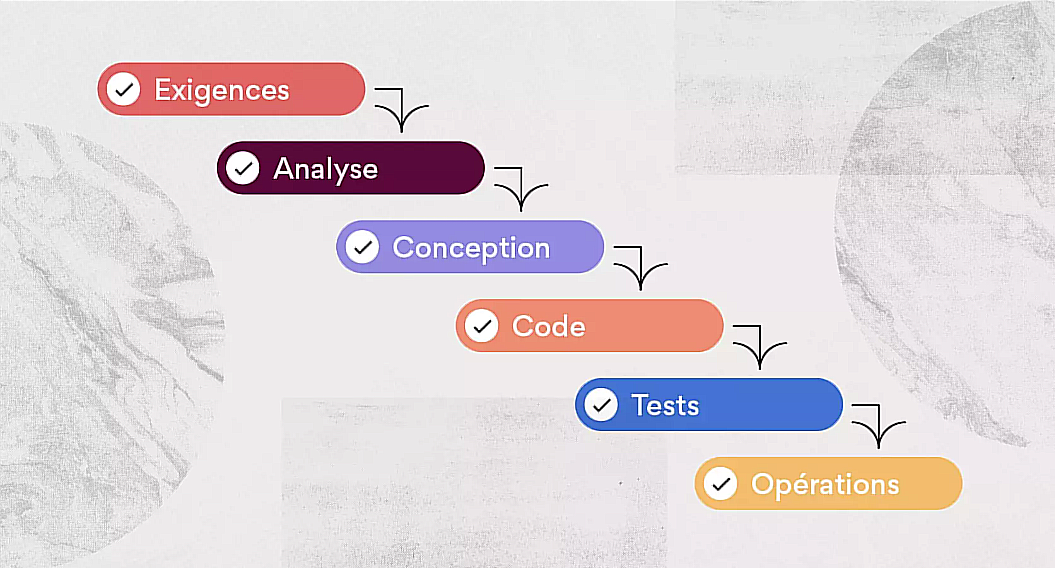
\includegraphics[width=0.9\textwidth]{pic/cascade.png} 
    \caption{Modèle en cascade}
    \label{Modèle en cascade}
\end{figure*}

Pour le semestre 9, on nous demande de nous concentrer sur la prise en main du sujet et la définition précise du travail à effectuer. Cela correspond aux tâches d'Exigences et d’Analyse.
J'ai cependant déjà pu m'avancer sur la partie Conception dès le mois de novembre comme nous le verrons dans la suite du rapport.
\end{itemize}

\chapter{Description générale}
\section{Environnement du projet}

L’environnement de développement est le suivant :
\begin{itemize}
    \item Le système d’exploitation : Windows;
    \item Le logiciel de modélisation : Gusek;
    \item Le matériel pour le développement : Machine personnelle ou PC fixe de Polytech\\
    \item L'IDE utilisé pour le développement : Visual Studio Code
\end{itemize}

Les différents acteurs du projet peuvent également être amenés à faire des réunions en présentiel ou visio par Teams pour discuter des contraintes à rajouter ou modifier, ou simplement s'échanger des mails.


\section{Caractéristiques des utilisateurs}

Seul l'étudiant ou l'encadrant sera amené à utiliser le logiciel tel quel, étant donné que son utilisation nécessite une connaissance approfondie du sujet et de l'informatique. Cependant les résultats obtenus seront des instructions à suivre et/ou des propositions d'organisation des échantillons à évaluer par le personnel des centres d'examen.
\pagebreak

\section{Fonctionnalités du système}
\subsection{Fonctionnalités du modèle}
Les fonctionnalités du modèle sont plutôt simples :

\begin{figure*}[h!]
    \centering
    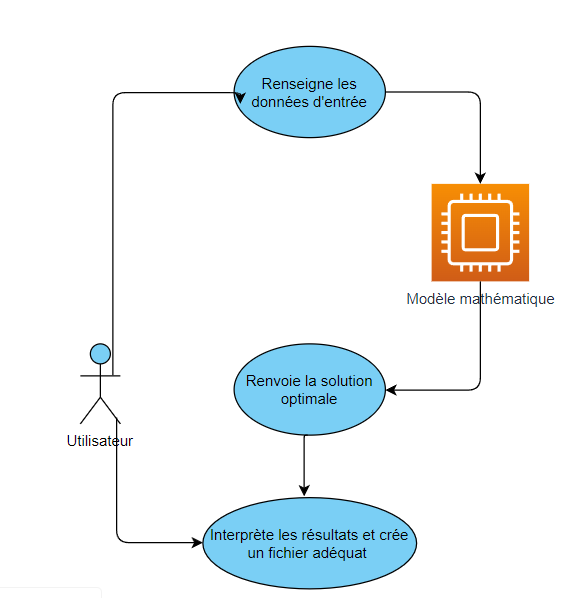
\includegraphics[width=0.9\textwidth, scale=0.8]{pic/usecasemodele.png}
    \caption{Diagramme de cas d'utilisation du modèle}
    \label{Diagramme de cas d'utilisation du modèle}
\end{figure*}

En pratique, les données d'entrée vont très peu changer : elles correspondent aux villes d'études (5 dans notre cas), et aux quantités produites et demandées d'échantillons de différents types pour chaque ville.

Si le système trouve une solution, les résultats envoyés seront les flux d'échantillons pour chaque ville, regroupés dans un grand tableau. On peut ensuite se servir de ces données pour imager le flux à réaliser et rédiger en conséquence la marche à suivre pour tous les centres d'analyse.

La partie Modélisation mathématique rentre plus en détail dans le fonctionnement du modèle implémenté.

\subsection{Fonctionnalités de l'application}

\begin{figure*}[h!]
    \centering
    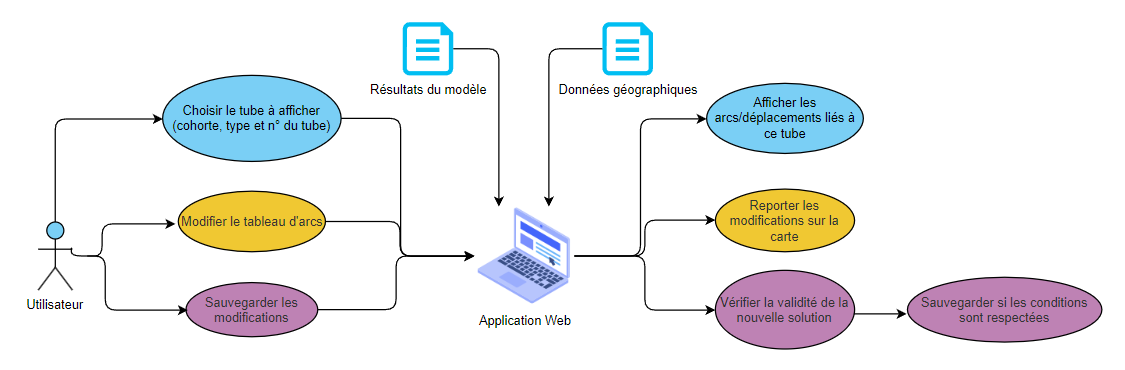
\includegraphics[width=0.9\textwidth]{pic/usecaseapp.png}
    \caption{Diagramme de cas d'utilisation de l'application}
    \label{Diagramme de cas d'utilisation de l'application}
\end{figure*}

L'application nécessite en entrée la solution proposée par le modèle, i.e le flux d'échanges pour tous les tubes. Il lui faut également des données géographiques afin d'initialiser la carte et poser des marqueurs sur les villes des centres d'analyse.

Après avoir sélectionné le tube, les arcs associés sont dessinés sur la carte et le tableau associé s'affiche afin de permettre la modification de la solution.

Enfin les conditions pour la sauvegarde visent à assurer que chaque centre soit desservi comme prévu (que la demande soit respectée), qu'il n'y ait pas de doublons, de boucle, ect...

\section{Structure générale du système}

Il n'y a que 2 composantes principales dans le système, à savoir : 
\begin{itemize}
    \item Le modèle construit sur Gusek, ou l'\gls{heuristique} de M.Billaut
    \item L'application web de visualisation
\end{itemize}

Il y a ensuite des fichiers/données d'entrée et de sortie pour chacun, notamment les variables de l'étude médicale et les coordonnées des centres d'analyse.

\begin{figure*}[h!]
    \centering
    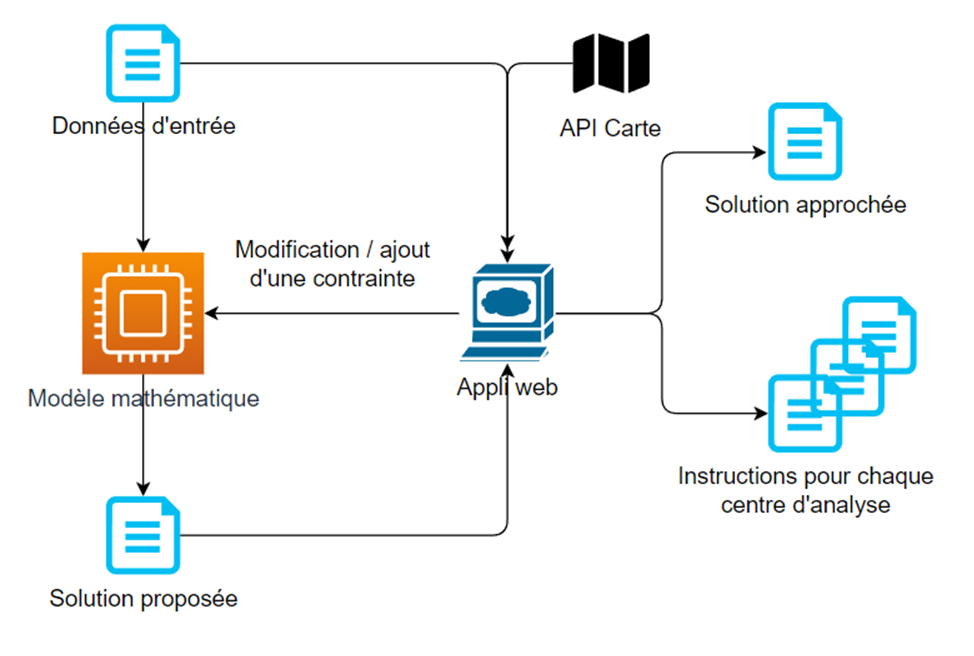
\includegraphics[width=0.9\textwidth, height=7cm]{pic/structuresysteme.png}
    \caption{Diagramme de la structure générale du système}
    \label{Diagramme de la structure générale du système}
\end{figure*}

\chapter{État de l'art / Veille technologique}

À notre connaissance, le problème n'a pas été abordé sous cet angle dans la recherche. Cependant il existe de nombreux articles concernant des problèmes similaires, que nous allons aborder ici.

\section{Voyageur de commerce et tournée de véhicule}

Le problème du voyageur de commerce (TSP en anglais pour Travelling Salesman Problem) est un problème très connu en informatique, et les algorithmes permettant sa résolution sont très documentés. Le problème de la tournée de véhicule (VRP en anglais pour Vehicle Routing Problem) est un dérivé du 1er, et les deux se présentent ainsi : 

\begin{figure*}[h]
    \centering
    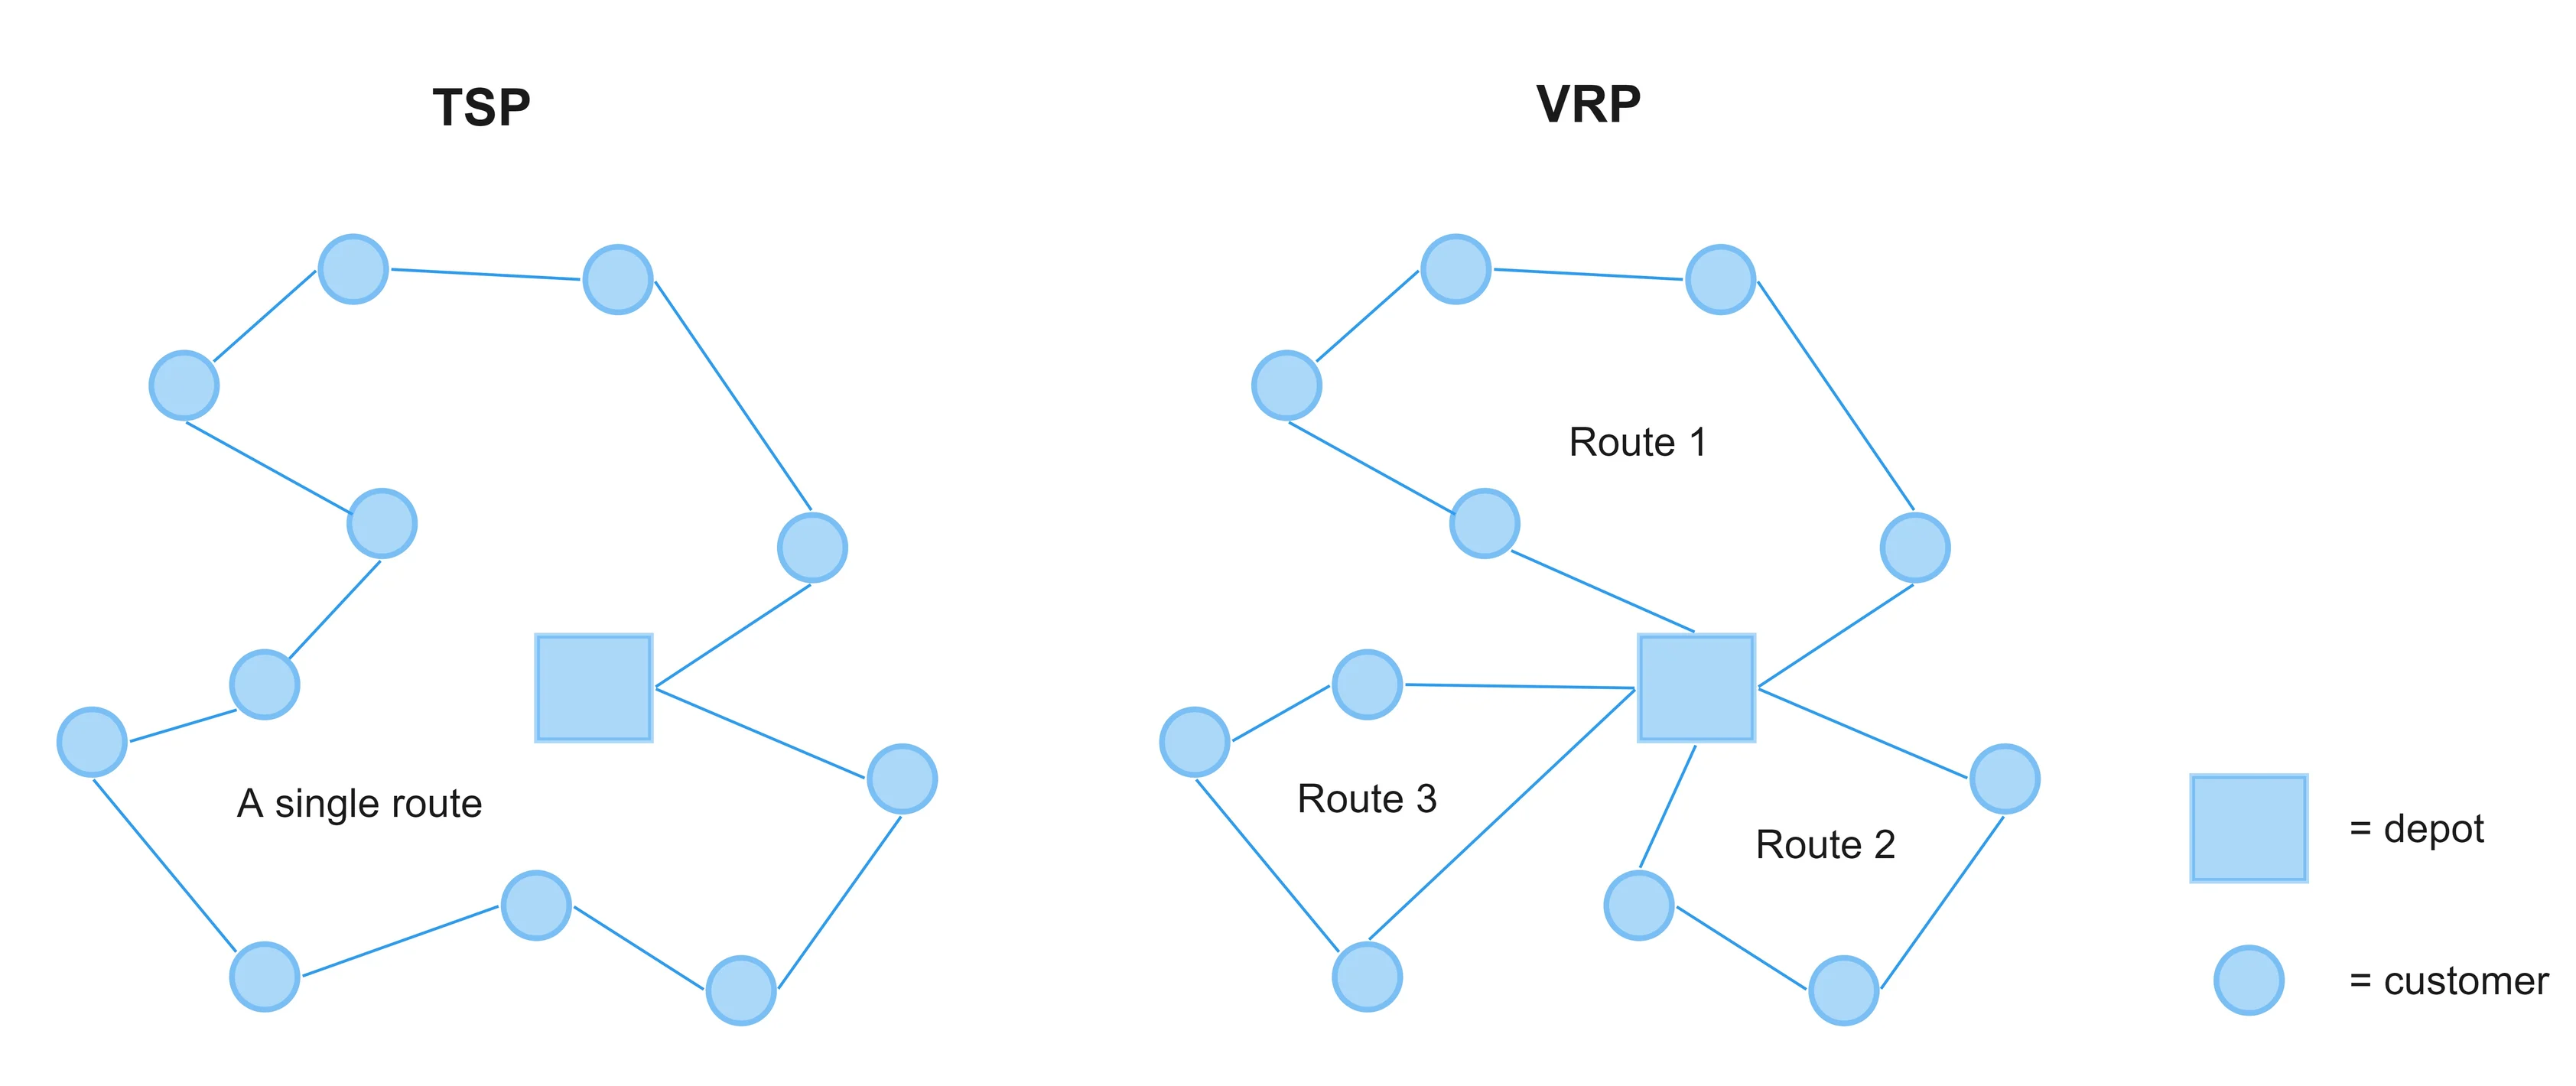
\includegraphics[width=0.9\textwidth]{pic/TSPVRP.png}
    \caption{Illustration DU TSP et VRP}
    \label{Illustration DU TSP et VRP}
\end{figure*}

Le TSP considère un ensemble de villes, où le but est de passer une seule et unique fois par chacune d'entre elles et de revenir au point de départ, en minimisant au maximum la distance du trajet parcouru.\\
Le VRP étend le problème à un ensemble de trajets et de véhicules, où l'objectif est d'affecter à chaque ressource un trajet permettant de couvrir l'ensemble des villes à traverser, tout en répartissant la charge de façon équitable entre toutes les ressources. 

Par exemple dans ce papier \cite{VRP}, les 3 chercheurs se focalisent sur la résolution d'un VRP où les "clients" sont des centres de collecte du sang et où le "dépôt" est le centre d'analyse. Ils utilisent pour cela différentes \glspl{heuristique} et les comparent entre elles, le but étant de trouver le nombre optimal de camions pour assurer au mieux la collecte et le transport des échantillons en respectant différentes contraintes de temps, d'argent et de conservation des échantillons sanguins.

Notre sujet prend en quelque sorte le problème du VRP à l'envers : Au lieu d'aller du client au dépôt comme dans la plupart des études concernant le transport d'échantillons de sang, on part du dépôt pour livrer tous les clients. Il conviendrait donc de replacer le mot "dépôt" par source qui fait plus de sens dans notre cas, ce qui nous donne un schéma comme cela : 

\begin{figure*}[h]
    \centering
    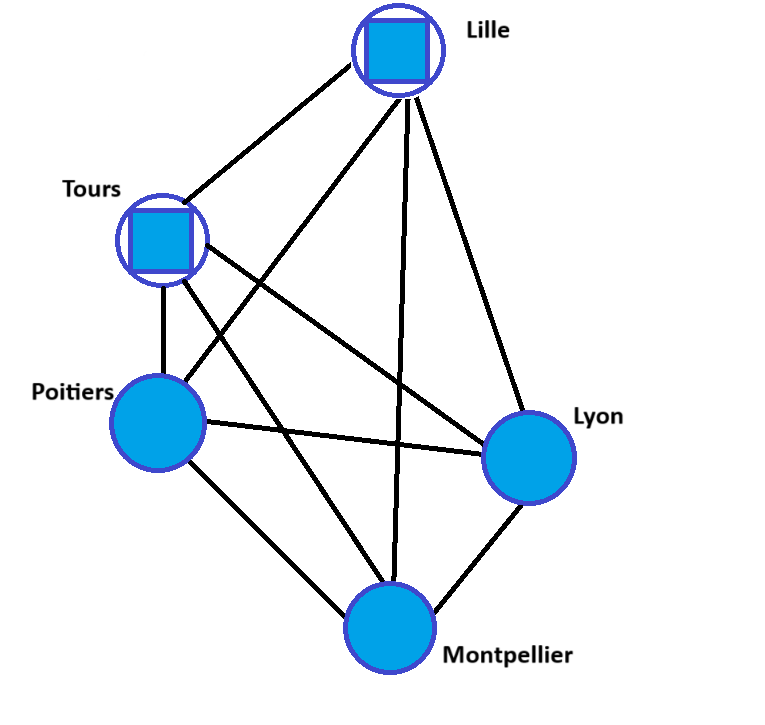
\includegraphics[width=0.9\textwidth]{pic/VRPPRD.png}
    \caption{Illustration du sujet sous la forme d'un VRP}
    \label{Illustration du sujet sous la forme d'un VRP}
\end{figure*}

On peut facilement mettre en lumière les différences entre les problèmes classiques de VRP et le nôtre : 
\begin{itemize}
	\item Comme dit plus haut on prend les routes "à l'envers".
	\item Il y a plusieurs sources, et une même route peut être empruntée par des échantillons provenant de sources différentes, ou au contraire utilisée par une seule source uniquement.
	\item L'échantillon n'a pas besoin de revenir au point de départ, puisqu'on considère que les cohortes se servent en premier avant de distribuer le reste des échantillons aux autres centres d'analyse.
\end{itemize}

Toutes ces raisons font que les méthodes de résolution classique du VRP ne peuvent pas s'appliquer à notre problème, ce qui implique de trouver de nouveaux algorithmes et méthodes de résolution.         
\chapter{Analyse et conception}
\section{Analyse}
\subsection{Explication du graphe}
Afin de modéliser correctement le modèle de façon mathématique, on a décidé de le représenter sous forme d'un graphe, où les villes représentent les sommets et les arcs correspondent à l'envoi d'échantillons d'une ville à l'autre.

En plus des 5 villes, on ajoute également 3 sommets "fictifs" : 
\begin{itemize}
	\item S : C'est le sommet Source, qui va envoyer aux 2 cohortes (ici Tours et Lille) les quantités initiales de chaque tube.
	\item OK : C'est le sommet qui représente l'utilisation des échantillons par une ville.
	\item P : C'est le sommet Puits, qui va recevoir toutes les quantités en trop non utilisées\\
\end{itemize}

On peut alors obtenir un graphe comme celui-ci :

\begin{figure*}[ht]
    \centering
    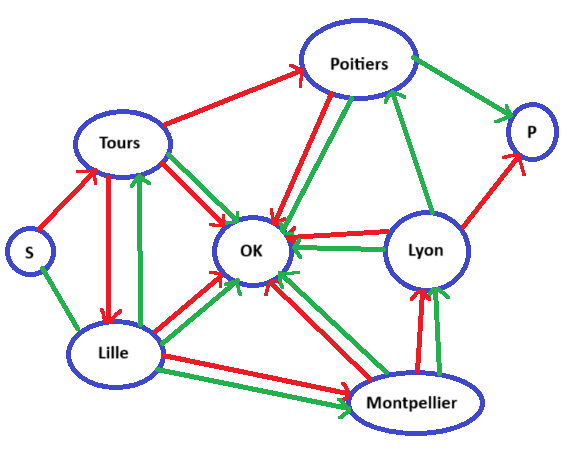
\includegraphics[width=0.7\textwidth, height=5cm]{pic/graph.png}
    \caption{Exemple de graphe possible}
    \label{Exemple de graphe possible}
\end{figure*}
\textcolor{red}{En rouge : Flux d'échantillons des patients de Tours}

\textcolor{green}{En vert : Flux d'échantillons des patients de Lille}\\

On aurait pu utiliser des arcs réflexifs (arc qui part d'un sommet et pointe vers le même sommet) pour dire qu'une ville utilise une partie des échantillons mais il était plus simple de faire ça avec un sommet bien distinct pour la création des contraintes du modèle (voir partie Modélisation mathématique).

\subsection{Contraintes imposées}
Le modèle à implémenter doit respecter un certain nombre de contraintes, fournies par Dr.BLASCO Hélène, vice-présidente de la recherche au CHRU de Tours.
Elles sont au nombre de 6 :
\begin{itemize}
	\item Tous les échantillons sont précieux, par conséquent il faut jeter le moins possible de sérum, plasma et liquide céphalo-rachidien.
	\item Prendre en compte le nombre de cycles congélation/décongélation de chaque tube et le minimiser. \\En effet les tubes doivent être congelés pour être transportés et décongelés pour pouvoir les analyser.
	\item Empêcher certaines analyses si tous les tubes n'ont pas le même nombre de cycle C/D.
	\item Limiter l'\gls{aliquotage} des tubes, car c'est une opération source d'erreurs.
	\item Intégrer une notion de temps aux analyses, car certaines sont plus longues que d'autres ou bien prioritaires.
	\item Enfin mixer des échantillons de Tours et de Lille dans les analyses afin qu'ils soient traités en même temps.\\

\end{itemize}

\section{Modélisation mathématique}
\subsection{Données}
\subsubsection{Données d'entrée constantes}

\begin{itemize}
	\item villes : Liste contenant les 5 villes : "Tours, Poitiers, Lyon, Lille, Montpellier".
	\item ville\_dep : Liste contenant les cohortes (ou villes de "départ") : "Tours, Lille".
	\item sp : Liste contenant les 3 sommets fictifs : "S, P, OK".
	\item typeTube : Liste contenant les 3 types d'échantillons : "PLA, SER, LCR" pour Plasma, Sérum et Liquide Céphalo-Rachidien.
	\item nbTubes : Tableau à 2 dimensions [ville\_dep, typeTube] d'entiers contenant le nombre de tubes d'un certain type prélevés par patient pour chaque cohorte.
	\item qtTubes : Tableau à 2 dimensions [ville\_dep, typeTube] de réels contenant la quantité prélevée d'un certain type de tube par patient pour chaque cohorte.
	\item demande : Tableau à 2 dimensions [villes, typeTube] de réels contenant les demandes en mL de chaque type de tube pour chacune des villes.
	\item HV : Réel arbitrairement grand nécessaire à l'écriture de certaines contraintes, strictement supérieure au flux maximum d'une ville à l'autre.
\end{itemize}

\subsubsection{Variables du modèle}

\begin{itemize}
	\item PhiT : Tableau à 4 dimensions [villes+sp, villes+sp, typeTube, nbTubes] de réels contenant la quantité envoyée d'un certain type de tube d'un patient de la cohorte de Tours d'une ville (ou sommet fictif) à une autre via un numéro de tube particulier.
Pour résumer, si on a PhiT["Tours", "Poitiers", "SER", "2"] = 0.2, cela signifie que Tours a envoyé à Poitiers 0.2mL de sérum via le tube n°2.
	\item PhiL : Même chose pour les patients de la cohorte de Lille.
	\item puits : Réel contenant la somme de tout ce qui a été jeté.
	\item congelT : tableau à 3 dimensions [villes, typeTube, nbTubes] de type booléen indiquant si le tube a subi un cycle C/D lors du départ de la ville.
	\item nbCongelT : tableau à 2 dimensions [typeTube, nbTubes] de réels comptant le nombre de congélations par tube.
	\item congelL : idem pour le flux de Lille.
	\item nbCongelL : idem pour le flux de Lille.
	\item envoiT : tableau à 4 dimensions [villes, villles, typeTube, nbTubes] de type booléen indiquant si une ville envoie quelque chose à une autre via un tube précis.
	\item aliT : tableau à 3 dimensions [villes, typeTube, nbTubes] d'entiers comptant le nombre d'aliquotages d'une ville pour un tube donné.
	\item envoiL : idem pour le flux de Lille.
	\item aliL : idem pour le flux de Lille.\\
\end{itemize}

Plutôt que d'utiliser 2 flux différents, on pourrait aussi pu rajouter une dimension de plus de taille ville\_dep. Cela est un choix arbitraire et il est tout à fait possible que l'on change la façon dont on définit le flux en fonction des contraintes et de la vitesse de résolution.

\subsection{Contraintes dîtes "de graphe"}

Ces contraintes forcent le modèle à respecter notre vision du problème en graphe. Certaines contraintes sont spécifiques à Tours, mais il suffit de les dupliquer pour Lille. Comme dit plus haut il est également possible de rassembler les 2 flux et de faire une contrainte plus générale en rajoutant une dimension.

\subsubsection{Contraintes de source}

Elles permettent d'initialiser les quantités d'échantillons pour toutes les villes : 

\begin{figure*}[ht]
    \centering
    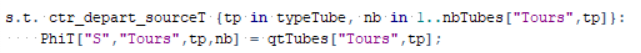
\includegraphics[width=\textwidth]{pic/source1.png}
    \caption{Contrainte de source (pour les cohortes)}
\end{figure*}

\begin{figure*}[ht]
    \centering
    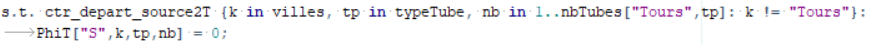
\includegraphics[width=\textwidth]{pic/source2.png}
    \caption{Contrainte de source (pour les autres villes)}
\end{figure*}

Pour chaque tube, le sommet Source envoie les quantités définies dans qtTubes pour les villes cohortes, et rien pour les autres.

\subsubsection{Contrainte de quantité max}

Elle permet de limiter le flux par rapport à la capacité max de chaque tube :

\begin{figure*}[ht]
    \centering
    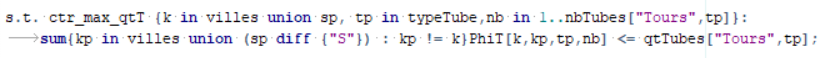
\includegraphics[width=\textwidth]{pic/maxqt.png}
    \caption{Contrainte de quantité maximum}
\end{figure*}

Pour chaque ville et chaque tube qu'elle envoie, la somme de tout ce qu'elle envoie d'un même tube ne peut pas dépasser la quantité initiale (définie dans qtTubes).  

\subsubsection{Contrainte de demande}

Elle permet de faire en sorte que la demande de chaque ville soit respectée :

\begin{figure*}[ht]
    \centering
    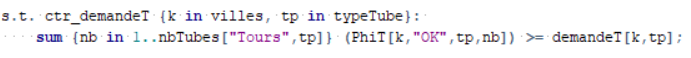
\includegraphics[width=\textwidth]{pic/demande.png}
    \caption{Contrainte de demande}
\end{figure*}

Pour chaque ville et chaque type de tube, la somme des quantités de chaque tube (du même type) envoyés au sommet OK doit être supérieure à la demande de la ville.

\subsubsection{Contrainte du puits}

Elle permet de définir la variable puits :\\ \\

\begin{figure*}[h]
    \centering
    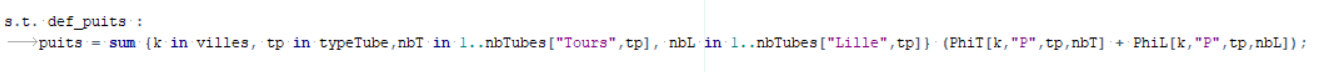
\includegraphics[width=\textwidth]{pic/puits.png}
    \caption{Contrainte du puits}
\end{figure*}

La variable puits est définie comme la somme de tout ce qu'envoie chaque ville au sommet P, tube et et type de tube confondu.

\subsubsection{Contraintes de boucles et flots}

Elles permettent de vérifier que les quantités envoyées soient égales aux quantités reçues

\begin{figure*}[ht]
    \centering
    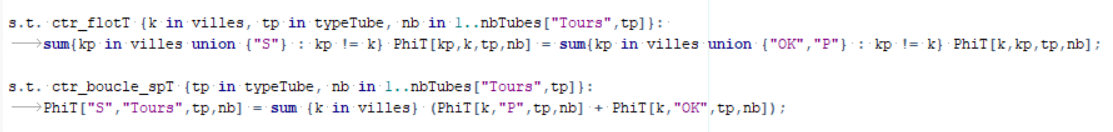
\includegraphics[width=\textwidth]{pic/flot.png}
    \caption{Contrainte de boucle et flot}
\end{figure*}

La contrainte de flot assure que pour chaque ville, la somme de ce qu'elle reçoit sur un tube est égale à la somme de ce qu'elle envoie de ce même tube.\\
La contrainte de boucle assure que pour chaque tube, la somme de ce qui est envoyé sur les sommets OK et P, toute ville confondue, est égale à la quantité initiale envoyée sur Tours. 
\pagebreak
\subsection{Contraintes imposées}

Ces contraintes forcent le modèle à respecter les attentes réelles des centres d'analyse : 

\subsubsection{Contraintes de congélation/décongélation}

Elles permettent de d'identifier si un tube a été congelé et de compter son nombre total de cycle C/D.

\begin{figure*}[ht]
    \centering
    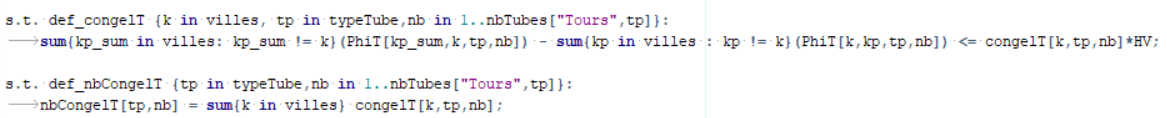
\includegraphics[width=\textwidth]{pic/congel.png}
    \caption{Contraintes de congélation/décongélation}
\end{figure*}

\paragraph{congelT}

La contrainte congelT est complexe à définir et ne prend pas en compte tous les cas de figure. Néanmoins elle fonctionne comme cela pour l'instant :\\
Pour chaque ville et chaque tube qu'elle envoie, la somme de tout ce qu'elle reçoit via d'autres villes sur ce tube \textbf{moins} la somme de tout ce qu'elle envoie aux autres villes (OK et P exclus !) depuis ce tube est inférieure ou égale à la variable de congélation de cette ville pour ce tube multiplié par HV (une très grande valeur).\\

L'idée derrière cette contrainte est si la somme de ce que la ville envoie est strictement comprise entre 0 et ce qu'elle reçoit, cela signifie que le tube a été décongelé pour pouvoir se servir, et recongelé pour envoyer le reste.
congelT étant une variable binaire, si la valeur à gauche est strictement supérieure à 0 alors congelT passera à 1 pour conserver l'égalité car 1*HV dépassera toujours le flux.

Il serait facile de définir congelT avec 2 contraintes différentes, mais la méthode de résolution de Gusek ne le permet pas (le programme tourne en boucle car valider une contrainte invalide l'autre).

\paragraph{nbCongelT}

nbCongelT est bien simple à définir car il suffit de calculer pour chaque tube combien de cycles C/D il a subi en additionnant tous les 1 de congelT pour ce tube.

\subsubsection{Contraintes d'aliquotage}

Elles permettent d'identifier si un tube a été aliquoté et de savoir en combien de tubes il a été séparé.
\begin{figure*}[ht]
    \centering
    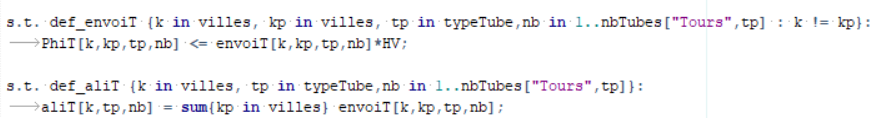
\includegraphics[width=\textwidth]{pic/aliquotage.png}
    \caption{Contraintes d'aliquotage}
\end{figure*}

\paragraph{envoiT}

envoiT est relativement simple à définir : pour chaque échange entre 2 villes différentes, si le flux est strictement positif alors envoiT est à 1, 0 sinon.

\paragraph{aliT}

De la même manière que nbCongelT, aliT compte le nombre d'envoi d'un tube depuis une même ville. A noter qu'il y a réellement \gls{aliquotage} à partir de aliT = 2.

\subsection{Fonction objectif}

La fonction objectif permet de donner un but au modèle.

On identifie en premier les variables présentes dans la fonction, à ce stade là du modèle cela comprend le nombre de cycles C/D, le nombre d'aliquots et la quantité de produits jetés.

\begin{figure*}[ht]
    \centering
    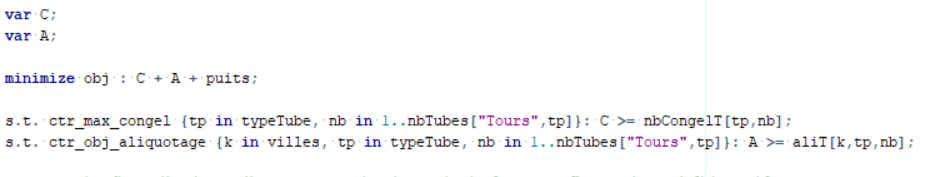
\includegraphics[width=\textwidth]{pic/objectif.png}
    \caption{Contrainte objectif}
\end{figure*}

On définit C et A respectivement comme le nombre max de cycles C/D et d'aliquots parmi tous les tubes, et on essaie de minimiser la somme des 3 variables avec le puits.\\
C'est une fonction objectif provisoire, car chaque variable est censée avoir un poids qui lui est associée pour définir un ordre de priorité. Par exemple il est peut-être plus important de limiter le nombre de cycles C/D quitte à augmenter l'\gls{aliquotage}.

\subsection{Amélioration du modèle}

Le modèle créé sur Gusek nous a permis d'avoir une vision plus précise du problème et des difficultés à prendre en compte. Il a cependant ses limites, que ça soit en termes de performances ou de structure générale.\\
C'est pourquoi M.Billaut et Mme.Vinot ont décidé de laisser le modèle Gusek tel quel afin de se concentrer sur l'élaboration d'heuristiques, qui pourraient résoudre plus intelligemment la répartition du flux d'échantillons en se servant notamment de nos réflexions conjointes sur le modèle initial.\\
Cela m'a également permis de passer à la 2ème partie du PRD, i.e. l'application de visualisation.

\section{Application de visualisation de la solution}

\subsection{Présentation générale}

L'outil de visualisation de la solution optimale a été développé sous la forme d'une application Web, disposant à  ce jour que d'une seule page principale. Cette page contient une carte interactive avec des marqueurs sur l'emplacement des centres d'analyse, un formulaire pour sélectionner le flux du tube à visualiser et enfin un tableau d'arcs qui se remplit adéquatement avec les informations du tube sélectionné.\\

\begin{figure*}[h]
    \centering
    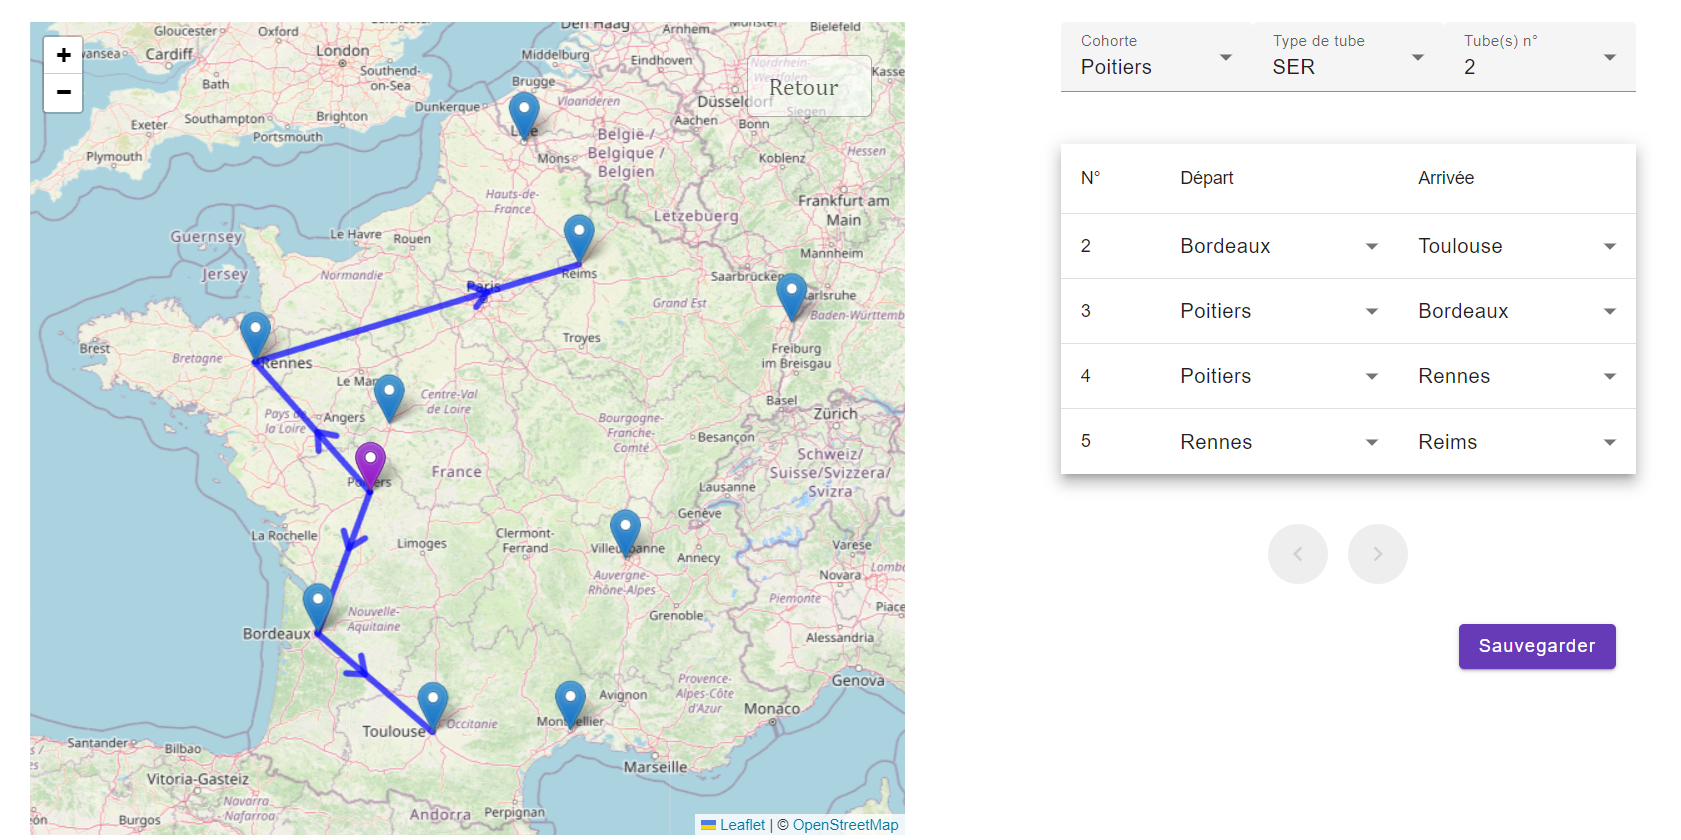
\includegraphics[width=0.9\textwidth]{pic/appweb.png}
    \caption{Page principale de l'application}
    \label{appweb}
\end{figure*}

Il est possible de modifier le départ et l'arrivée de chaque arc via les listes déroulantes dans le tableau, et de voir les arcs sur la carte être modifiés adéquatement.

Le bouton "Sauvegarder" permet de vérifier que les modifications apportées à la solution soient cohérentes et réalisables (pas de boucle, demande de chaque centre respectée,...), et affiche un message d'erreur ou de réussite en fonction du résultat.\\
Il n'y a pas de véritable sauvegarde des modifications, mais nous y reviendrons plus tard dans les difficultés rencontrées. 

\subsection{Structure de l'application}

L'application a été développée en Angular, ce qui impose de réfléchir en termes de composants. Ainsi j'ai décidé de développer 3 composants différents, un principal contenant la carte et 2 autres composants dits "enfants" contenant respectivement le formulaire de sélection du tube et le tableau d'arcs (avec le bouton sauvegarder).\\

La notion de composant enfant et parent permet une communication entre eux et de passer en paramètre des données initialisées dans un composant externe. De plus, Angular permet de développer des "services" permettant une connexion plus générale entre tous les composants indifféremment des relations enfant/parent, tout en factorisant des méthodes coûteuses en temps de calcul.\\
L'application contient donc 2 services, 1 pour la construction d'un objet JSON de la solution à partir des données d'entrée et de sortie du modèle, et 1 autre pour l'affichage des arcs à la fois sur la carte et dans le tableau. Nous reviendrons plus en détail sur la construction de la solution.\\

Voici un schéma représentant la structure de l'application :

\begin{figure*}[h]
    \centering
    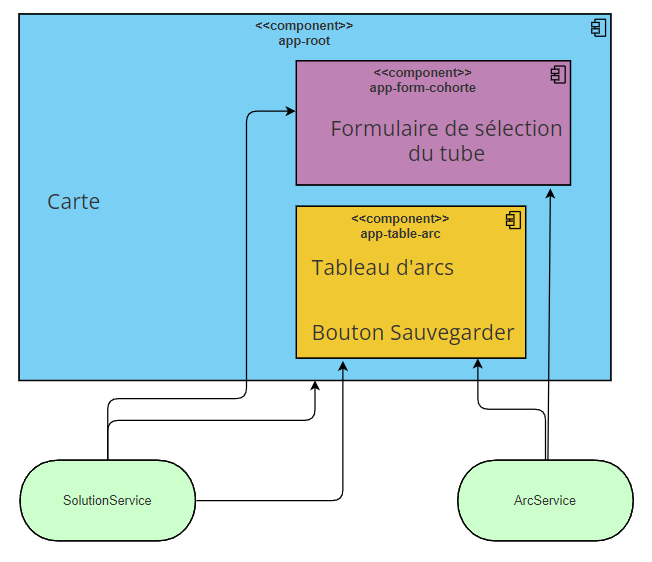
\includegraphics[width=0.9\textwidth]{pic/structureapp.png}
    \caption{Structure de l'application}
\end{figure*}

\subsubsection{SolutionService}

Le service Solution gère la plupart des fonctionnalités de l'application et il est relativement dense, notamment à cause des 3 fichiers d'entrée différents qu'il utilise :\\

\begin{itemize}
	\item map.geojson : Ce fichier contient la liste des villes qu'on devra afficher sur la carte, avec leurs coordonnées géographiques. Il a été créé de façon arbitraire par moi-même via un site internet. Cela signifie qu'il faudra recréer le fichier de toutes pièces si l'on veut changer les villes d'exemple.
	\item instance.txt : C'est le fichier d'entrée de l'heuristique, qui précise entre autres le nombre de villes et de types de prélèvements, et la demande de chaque centre.
	\item solution\_instance.txt :C'est le fichier de sortie de l'heuristique i.e. la solution optimale, qui à ce jour contient uniquement la répartition des villes et des échanges entre les tubes. Par exemple le tube n°2 de sérum de la cohorte de Poitiers (coir image) \ref{fig:appweb} fera le lien entre les villes de Poitiers, Bordeaux, Toulouse, rennes et Reims.\\
    Il n'y a cependant pas encore de notion de quantité envoyée ou de nombre d'aliquots, uniquement la liste des villes desservies pour chaque tube.\\
\end{itemize}

\pagebreak

La fonction parseSolution() est la méthode principale du service avec presque une centaine de lignes, qui se charge de créer un objet JSON structuré comme tel:

\begin{figure*}[h]
    \centering
    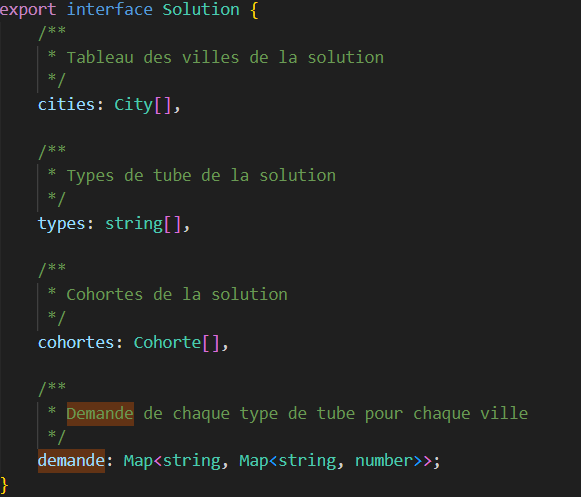
\includegraphics[width=0.9\textwidth]{pic/interfacesolution.png}
    \caption{Structure de l'objet Solution}
\end{figure*}

Le paramètre important ici est le tableau de cohortes, qui va contenir une ville cohorte et un tableau de Type, où chaque Type est composé d'un nom (LCR, SER, ...) et d'un tableau de Tube, où chaque Tube va être composé d'un numéro, d'un volume donné et d'une liste d'arcs correspondant à la répartition énoncée plus haut.\\

Les objets Solution, City, Cohorte, Type, Tube et Arc sont encapsulés dans des interfaces afin de permettre une meilleure lisibilité et d'être plus facilement modifiables, si par exemple on, souhaite rajouter un champ pour chaque Tube.\\

Le soucis dans la fonction parseSolution() est qu'elle est complètement dépendante de la nomenclature des fichiers d'entrée. On les parcourt ligne par ligne et la moindre modification dans la structure de ces fichiers imposerait de redévelopper la fonction en détail.\\

Cependant le développement en service Angular nous permet de gagner beaucoup de temps de calcul. En effet, la solution est construite une seule fois lors de l'ouverture de l'application, puis chaque composant va lire et modifier la même instance de l'objet ou une copie, mais sans avoir à tout recalculer.
Le service Arc fonctionne sur le même principe, mais il permet de "notifier" les composants lors d'une modification du tableau d'arcs afin qu'elle se répercute à la fois dans le tableau et sur la carte.

\subsection{Documentation et commentaires}

Nous savions depuis le début de l'année que ce projet allait être repris, ainsi l'accent a été mis sur la rédaction d'une documentation complète à fournir au prochain étudiant en parallèle du développement de l'application, visant à faciliter la reprise du sujet et du code. Ce rapport en fait partie, mais j'ai également généré une documentation détaillée de l'ensemble du code grâce à l'outil Compodoc, et accessible via une ligne de commande précisée dans le README du répertoire Git, avec d'autres instructions sur l'installation du projet notamment.\\

Cette documentation précise le but de chaque fonction, le type de leurs paramètres et les membres de chaque classe et chaque interface. Elle se présente comme cela:

\begin{figure*}[h]
    \centering
    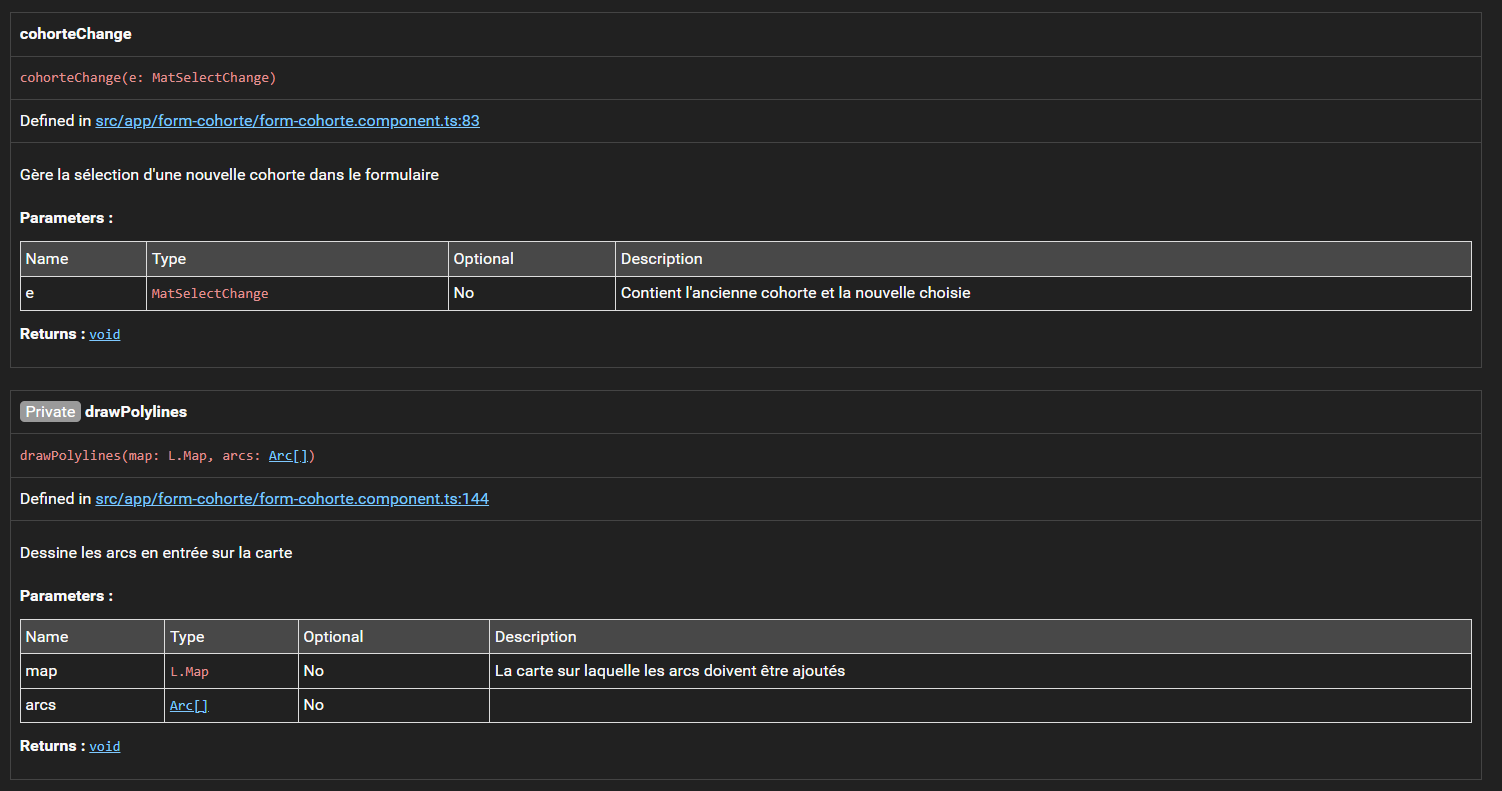
\includegraphics[width=0.9\textwidth]{pic/compodoc.png}
    \caption{Exemple de documentation du code avec Compodoc}
\end{figure*}

De plus, certaines parties complexes à appréhender dans le code sont commentées afin de faciliter au mieux la compréhension de celles-ci.
Enfin, j'ai rajouté des commentaires "TODO :", pour indiquer les fonctionnalités à compléter, à améliorer ou à créer. Il existe une extension sur Visual Studio Code (TodoTree) qui permet de voir tous les "TODO :" du projet sous la forme d'une liste déroulante, il est ainsi facile de voir par où commencer.

\subsection{Difficultés rencontrées}

La difficulté majeure du développement de cette application est liée à la nomenclature des fichiers d'entrée. Les informations du modèle sont de simples fichiers texte écrits "à la main", avec beaucoup de chiffres et peu de façons de les agencer de façon lisible et pratique à parcourir via le code. Peut-être qu'un autre format de fichier à l'avenir pourrait être une bonne idée, ou au moins un intermédiaire entre la sortie du modèle et l'entrée de l'application pour formaliser les données, ce qui permettrait également de rassembler les 3 fichiers dans un seul.\\

Le fichier de sortie du modèle aka la solution est également incomplète, car comme dit plus haut on dispose pour l'instant uniquement de la répartition des villes dans chaque tube, sans avoir des quantités précises échangées entre chacune d'entre elles. M.Billaut a développé plusieurs heuristiques avec chacune leur fonction, mais il n'a pas eu le temps de les combiner en un fichier de solution utilisable par l'application.\\

Cela a aussi un impact sur le développement du lien entre le modèle et l'application. En effet, elle ne dispose pas encore de Backend qui pourrait permettre une communication via une base de données, les fichiers d'entrée présents dans l'archive m'ont été envoyés par mail. Nous n'avons à la fois pas de moyen de comparer la différence entre la solution optimale et celle modifiée par l'utilisateur à cause du manque d'un format de fichier commun, ni un moyen d'exécuter une heuristique via l'application.\\ 

Enfin, à cause du temps relativement court pour développer l'application (à partir de fin janvier donc environ 2mois), j'ai décidé de ne pas faire de cahier de spécifications afin de gagner du temps, d'autant plus que M.Billaut m'avait donné "carte blanche" en termes de visuels. Cela m'a permis de gagner du temps sur les fonctionnalités développées mais j'en ai aussi perdu en tâtonnant entre différentes façons de modéliser le problème, avant de me concentrer sur la partie visualisation et de laisser la partie lien modèle/application pour plus tard.

\chapter{Bilan du PRD}

\section{Semestre 9}

Toute la partie de prise en main du sujet et la rédaction du cahier des spécifications s'est déroulée sans accroc et même avec un peu d'avance, étant donné qu'il n'y avait pas énormément de documentation à consulter et que le 1er modèle imaginé possède peu de fonctionnalités.\\
Cependant la 2ème modélisation avec la contrainte de congélation a pris plus de temps que prévu, suite à des difficultés liées à l'écriture des contraintes et la façon dont Gusek fonctionne, entraînant des retards sur le début du S10.\\
Ce n'est que mi-janvier que j'ai réussi à avoir un modèle cohérent et assez satisfaisant vis à vis des contraintes initiales, et que M.Billaut et Mme.Vinot ont décidé de s'occuper de la suite du modèle à l'aide d'heuristiques afin que je puisse entamer le développement de l'application.

\section{Semestre 10}

Bien que le semestre 10 ait commencé avec des retards par rapport au planning initial, et malgré le temps restant assez court pour le reste du projet, la majorité des attendus de l'application ont été réalisés de façon satisfaisante et prometteuse pour la suite de ce projet.\\
La documentation du code et du fonctionnement général du système modèle/visualisation a été menée à bien, je considère donc ce PRD comme une réussite personnelle et j'espère le voir un jour utilisé au sein de recherches médicales. 

\begin{appendix}
\selectlanguage{french}

\chapter{Planification, gestion de projet}   

\section{Évolution du projet}

Le diagramme de Gantt initial pour le S9:
\begin{figure*}[ht]
    \centering
    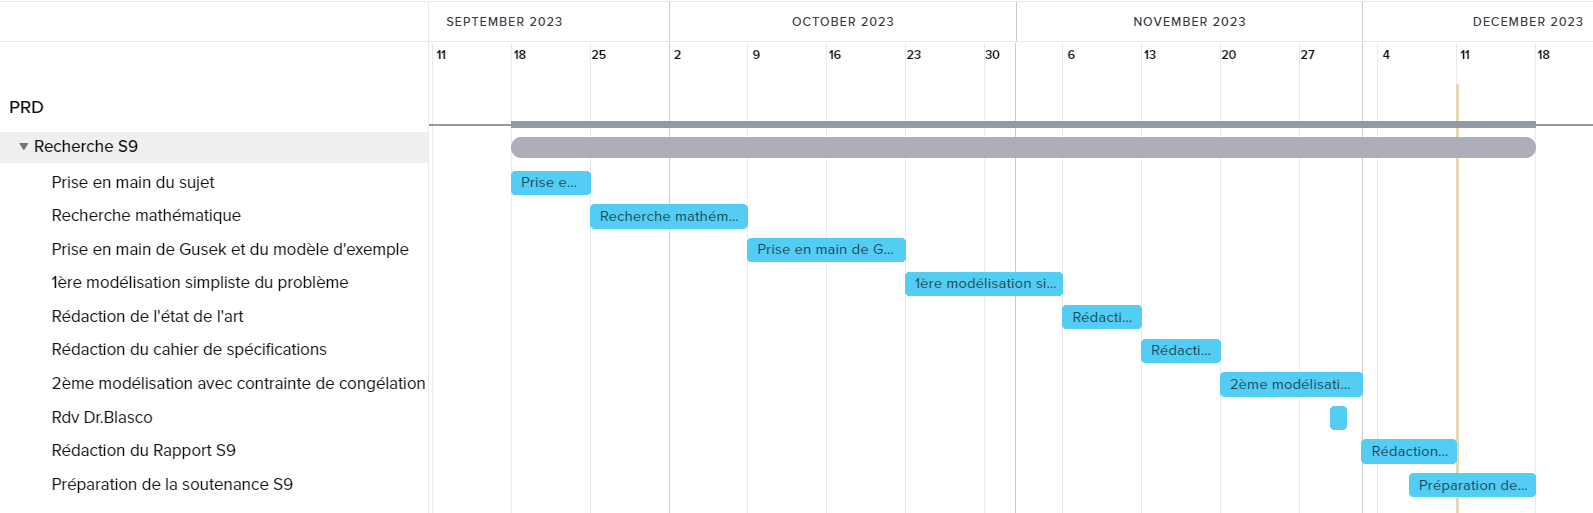
\includegraphics[width=\textwidth]{pic/gantts91.png}
    \caption{Diagramme de Gantt initial (S9)}
\end{figure*}

Le diagramme de Gantt final pour le S9 :
\begin{figure*}[ht]
    \centering
    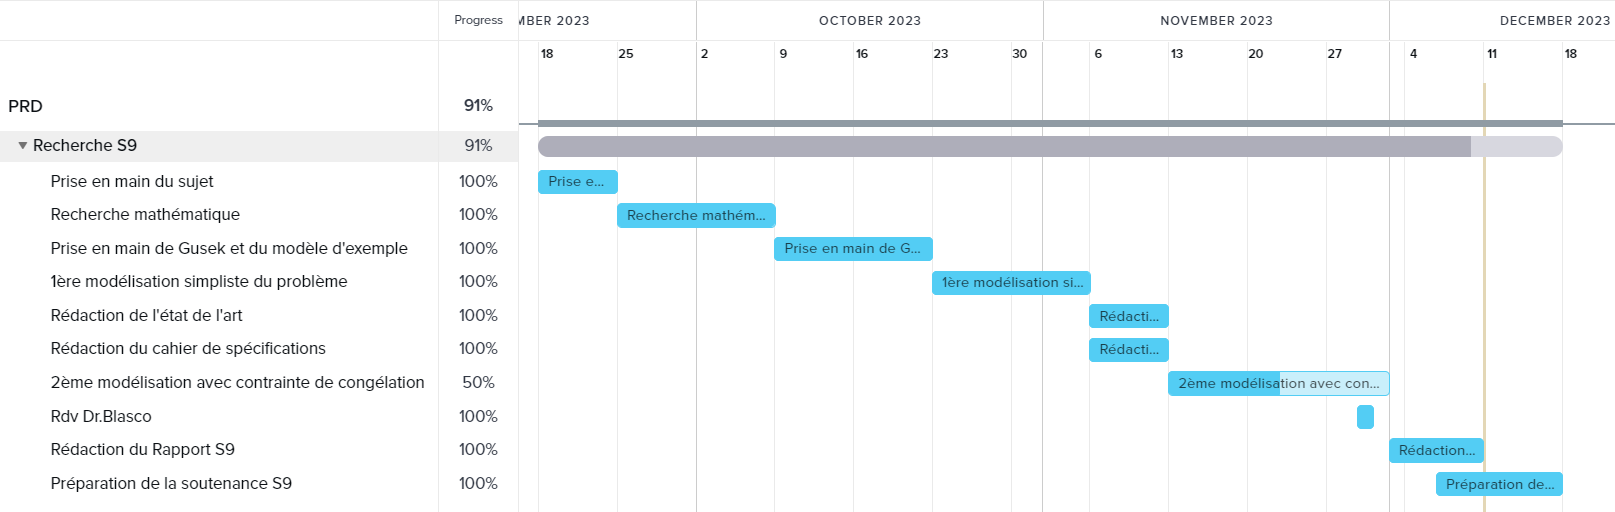
\includegraphics[width=\textwidth]{pic/gantts92.png}
    \caption{Diagramme de Gantt final (S9)}
\end{figure*}

Comme dit dans le bilan, la rédaction de l'état de l'art et du cahier de spécifications s'est avérée plus courte que prévue, ce qui m'a permis de commencer la 2ème modélisation plus tôt.\\
Malgré cela j'ai quand même pris du retard sur le S10 car je n'ai pas réussi à faire en sorte que la modélisation soit fonctionnelle et complète avant la soutenance.
Dans l'ensemble j'ai plutôt bien respecté le planning initial.\\

Pour le semestre 10, il n'y a pas vraiment eu de Gantt initial, j'ai très rapidement commencé à développer et je n'avais pas de sprints ou de livrables à donner avec des deadlines, le diagramme de Gantt suivant est un résumé de mon organisation pour ce semestre:

\begin{figure*}[ht]
    \centering
    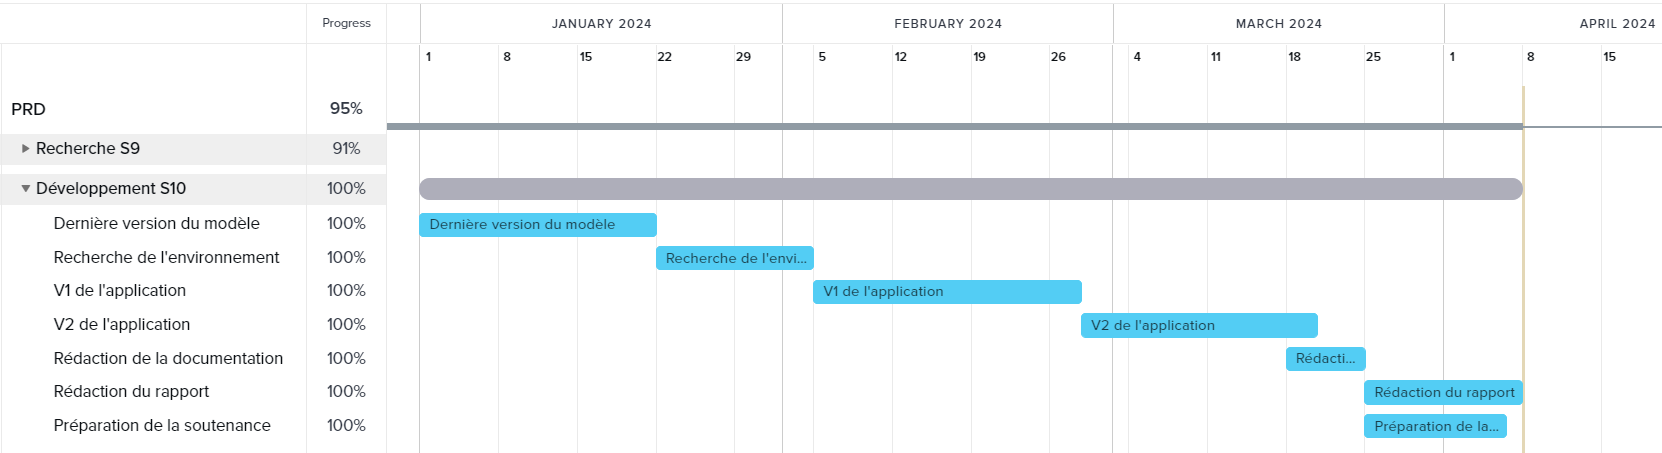
\includegraphics[width=\textwidth]{pic/gantts10.png}
    \caption{Diagramme de Gantt (S10)}
\end{figure*}

La dernière version du modèle m'a pris une grande partie du mois de janvier, et j'ai enchaîné avec la recherche de l'environnement de développement qui a pris un peu plus de temps que voulu, comme expliqué plus bas dans la description de la tâche.

\section{Description des tâches}

\paragraph{Tâche 1: Prise en main du sujet}

\begin{itemize}
    \item Date de début: 18/09/2023
    \item Date de fin: 25/09/2023
    \item Durée: 1 semaine
    \item
        Description: Lecture du sujet et des documents fournis, recherche des termes médicaux spécifiques (aliquotage...).
\end{itemize}

\paragraph{Tâche 2: Recherche mathématique}

\begin{itemize}
    \item Date de début: 25/09/2023
    \item Date de fin: 09/10/2023
    \item Durée: 2 semaines
    \item
        Description: Recherche internet des différents concepts mathématiques du sujet : Théorie des graphes, TSP, recherche opérationnelle. Renseignements sur la programmation par contraintes.
\end{itemize}

\paragraph{Tâche 3: Prise en main de Gusek et du modèle d'exemple}

\begin{itemize}
    \item Date de début: 09/10/2023
    \item Date de fin: 23/10/2023
    \item Durée: 2 semaines
    \item
        Description: Compréhension du modèle d'exemple fourni par M.Billaut : fonctionnement, variables utilisées, définition des contraintes,...\\
        Premiers tests sur Gusek avec des codes d'exemples et sur le modèle même.
        
\end{itemize}

\paragraph{Tâche 4: 1ère modélisation du problème}

\begin{itemize}
    \item Date de début: 23/10/2023
    \item Date de fin: 06/11/2023
    \item Durée: 2 semaines
    \item
        Description: Réparation des bugs présents dans le modèle initial fourni et développement d'une première version du modèle simpliste.\\
        Discussion avec M.Billaut sur la suite du modèle.
\end{itemize}

\paragraph{Tâche 5: Rédaction de l'état de l'art}

\begin{itemize}
    \item Date de début: 06/11/2023
    \item Date de fin: 13/11/2023
    \item Durée: 1 semaine
    \item
        Description: Recherche internet sur les papiers concernant le VRP et les études dans l'organisation d'échantillons médicaux, puis rédaction de l'état de l'art.
\end{itemize}

\paragraph{Tâche 6: Rédaction du cahier de spécifications}

\begin{itemize}
    \item Date de début: 06/11/2023
    \item Date de fin: 13/11/2023
    \item Durée: 1 semaine
    \item
        Description: Rédaction du cahier de spécifications grâce à la liste des contraintes fournie en début de projet.
\end{itemize}

\paragraph{Tâche 7: 2ème modélisation avec contrainte de congélation}

\begin{itemize}
    \item Date de début: 13/11/2023
    \item Date de fin: 04/12/2023
    \item Durée: 3 semaines
    \item
        Description: Développement d'un 2ème modèle qui intègre la contrainte de congélation, en essayant d'appliquer les idées qui suivaient les réunions avec M.Billaut. Cette tâche n'a pas été terminée dans les temps.
\end{itemize}

\paragraph{Tâche 8: Rendez-vous avec Dr.Blasco}

\begin{itemize}
    \item Date de début: 29/11/2023
    \item Date de fin: 29/11/2023
    \item Durée: 1 jour
    \item
        Description: Rendez-vous avec le Dr.Blasco pour discuter du sujet, de son avancée et comparaison entre les résultats donnés par les 1ers modèles et ses attentes. Explication de l'organisation actuelle de la distribution des échantillons.  
\end{itemize}

\paragraph{Tâche 9: Rédaction du Rapport S9}

\begin{itemize}
    \item Date de début: 04/12/2023
    \item Date de fin: 10/12/2023
    \item Durée: 6 jours
    \item
        Description: Rédaction de ce rapport
\end{itemize}

\paragraph{Tâche 10: Préparation de la soutenance S9}

\begin{itemize}
    \item Date de début: 06/12/2023
    \item Date de fin: 13/12/2023
    \item Durée: 1 semaine
    \item
        Description: Création du support pour la soutenance du semestre 9 et préparation de la soutenance en elle-même. 
\end{itemize}

\paragraph{Tâche 11: Dernière version du modèle}

\begin{itemize}
    \item Date de début: 01/01/2024
    \item Date de fin: 19/01/2024
    \item Durée: 3 semaines
    \item
        Description: Développement de la version finale du modèle, fonctionnelle avec les contraintes de congélation et d'\gls{aliquotage}. Par la suite, la solution provient des \glspl{heuristique} développées par M.Billaut. 
\end{itemize}

\paragraph{Tâche 12: Recherche de l'environnement}

\begin{itemize}
    \item Date de début: 22/01/2024
    \item Date de fin: 02/02/2024
    \item Durée: 2 semaines
    \item
        Description: Recherche de l'environnement de développement idéal.
        En 1er lieu je cherchais à faciliter la connexion entre l'outil de visualisation et le modèle, avant de me concentrer sur l'application afin d'avoir rapidement un visuel de la solution. J'avais privilégié une application "bureau" en C\# par exemple, mais je me suis rabattu sur du développement web puis du Angular vu mon expérience avec ce framework.
\end{itemize}

\paragraph{Tâche 13: V1 de l'application}

\begin{itemize}
    \item Date de début: 05/02/2024
    \item Date de fin: 27/02/2024
    \item Durée: 3 semaines
    \item
        1ère version simplifiée de l'application, comprenant la carte interactive avec un formulaire incomplet, pouvant afficher des arcs entre différents villes en fonction du choix. Il n'y avait pas encore de lien avec les fichiers d'entrée et de sortie du modèle/heuristique. 
\end{itemize}

\paragraph{Tâche 13: V2 de l'application}

\begin{itemize}
    \item Date de début: 28/02/2024
    \item Date de fin: 19/03/2024
    \item Durée: 3 semaines
    \item
        2ème version de l'application, comprenant la carte interactive avec un formulaire exhaustif, et un tableau d'arcs qui s'initialise de façon dynamique avec le choix du formulaire. L'application prend en entrée les 3 fichiers mentionnés plus haut, mais ne permet pas une communication avec le modèle directement. 
\end{itemize}

\paragraph{Tâche 14: Rédaction de la documentation}

\begin{itemize}
    \item Date de début: 18/03/2024
    \item Date de fin: 22/03/2024
    \item Durée: 1 semaine
    \item
        Rédaction de la documentation du code avec Compodoc, et rajout de commentaires et de TODO pour faciliter la lecture et la reprise du projet.
\end{itemize}

\paragraph{Tâche 15: Rédaction du rapport}

\begin{itemize}
    \item Date de début: 25/03/2024
    \item Date de fin: 05/04/2024
    \item Durée: 2 semaines
    \item
        Rédaction de ce rapport.
\end{itemize}

\paragraph{Tâche 16: Préparation de la soutenance}

\begin{itemize}
    \item Date de début: 25/03/2024
    \item Date de fin: 04/04/2024
    \item Durée: 2 semaines
    \item
        Préparation pour la soutenance finale de ce PRD.
\end{itemize}

\chapter{Cahier de Spécifications}

\section{Spécifications fonctionnelles}
Il n'y a que 3 fonctionnalités à développer pour le modèle, à savoir : 
\begin{itemize}
    \item Lecture des fichiers d'entrée
    \item Résolution du modèle
    \item Création des fichiers de sortie
\end{itemize}

Pour l'outil de visualisation, elles sont au nombre de 5:
\begin{itemize}
    \item Création d'un objet Solution
    \item Permettre la sélection d'un tube
    \item Afficher les arcs liés au tube choisi
    \item Pouvoir modifier les arcs d'un tube
    \item Sauvegarder les modifications
\end{itemize}

%~ \setcounter{secnumdepth}{2}
%~ \renewcommand\thesection{\arabic{section}} 

\subsection{ Définition de la fonction 1 : Lecture des fichiers d'entrée}

\paragraph{Description de la fonction 1 :}
 
\begin{description}
    \item[Lecture du fichier d'entrée] ~ \\
        Entrée : Fichier de données contenant :
        \begin{itemize}
            \item les villes,
            \item les cohortes parmi ces villes,
            \item les types d'échantillons prélevés,
            \item pour chacune des cohortes le nombre de tubes prélevés de chaque type par patient et la quantité en mL de chacun de ces tubes. 
        \end{itemize} \\
        Sortie : Rien
        Pré-conditions : Le fichier doit être conforme (bon format, bonne nomenclature, ect...) \\
        Post-conditions : Rien
\end{description}

\pagebreak

\subsection{Définition de la fonction 2 : Résolution du modèle}

\paragraph{Description de la fonction 2:}

\begin{description}
    \item[Variables d'entrée] ~ \\
        Entrée : Données du fichier d'entrée.\\ 
        Sortie : Variables initialisées\\
        Pré-conditions : Aucune \\
        Post-conditions : Les variables ont le bon type et la bonne dimension.

    \item[Résolution du modèle] ~ \\
        Entrée : Variables initialisées.\\ 
        Sortie : Variables du modèle après résolution\\
        Pré-conditions : Le modèle doit être solvable en temps acceptable\\
        Postconditions : Aucune
\end{description}

\subsection{Définition de la fonction 3 : Création des fichiers de sortie}

\paragraph{Description de la fonction 3:}

\begin{description}
    \item[Variables de sortie] ~ \\
        Entrée : Variables du modèle après résolution\\ 
        Sortie : Fichiers de résultats\\
        Pré-conditions : Le modèle n'a pas échoué \\
        Post-conditions : Les résultats sont écrits sur plusieurs fichiers différents, un pour chaque contrainte majeure (on écrit le contenu de chaque variable importante dans le fichier correspondant) .

    \item[Analyse des résultats] ~ \\
        Entrée : Fichiers de résultats.\\ 
        Sortie : Fichiers d'instructions à suivre et graphe correspondant à la répartition des échantillons \\
        Pré-conditions : Aucune\\
        Post-conditions : Aucune
\end{description}

\subsection{Définition de la fonction 4 : Création d'un objet Solution}

\paragraph{Description de la fonction 4:}

\begin{description}
    \item[Fichiers d'entrée] ~ \\
        Entrée : Fichier d'entrée et de sortie du modèle + la liste des villes à afficher.\\ 
        Sortie : Rien.\\
        Pré-conditions : Les fichiers doivent être récupérés et rangés dans les dossiers assets/map\_data et assets/solution\__data\\
        Post-conditions : Aucune.

    \item[Création de la solution] ~ \\
        Entrée : Les fichiers d'entrée.\\ 
        Sortie : Un objet JSON de type Solution\\
        Pré-conditions : Aucune.\\
        Postconditions : L'objet est correctement rempli avec les informations requises (répartition des tubes, demande, nom des villes,...)
\end{description}

\subsection{Définition de la fonction 5 : Permettre la sélection d'un tube}

\paragraph{Description de la fonction 5:}

\begin{description}
    \item[Sélectionner un tube] ~ \\
        Entrée : Aucune.\\ 
        Sortie : Un objet de type Tube.\\
        Pré-conditions : Le formulaire est initialisé grâce à l'objet Solution.\\
        Postconditions : La variable "tube" du composant app-forme-cohorte est initialisée avec l'objet Tube choisi.
\end{description}

\subsection{Définition de la fonction 6 : Afficher les arcs d'un tube choisi}

\paragraph{Description de la fonction 6:}

\begin{description}
    \item[Afficher les arcs d'un tube] ~ \\
        Entrée : Un objet de type Tube.\\ 
        Sortie : Aucune.\\
        Pré-conditions : Le tube est initialisé depuis la sélection du formulaire.\\
        Postconditions : Les arcs du tube choisi sont dessinés sur la carte et sont affichés dans le tableau d'arcs.
\end{description}

\subsection{Définition de la fonction 7 : Pouvoir modifier les arcs d'un tube}

\paragraph{Description de la fonction 7:}

\begin{description}
    \item[Modifier les arcs d'un tube] ~ \\
        Entrée : Un objet de type Tube.\\ 
        Sortie : La liste d'arcs modifiée du tube choisi.\\
        Pré-conditions : Le tableau d'arcs est initialisé avec les arcs du tube choisi.\\
        Postconditions : Les modifications effectués sur le tableau sont reportées sur la carte (les flèches sont mises à jour adéquatement).
\end{description}

\subsection{Définition de la fonction 8 : Sauvegarder les modifications}

\paragraph{Description de la fonction 8:}

\begin{description}
    \item[Sauvegarder les modifications apportées aux arcs d'un tube] ~ \\
        Entrée : La liste d'arcs modifiée d'un tube.\\ 
        Sortie : Un objet Solution contenant les nouveaux arcs.\\
        Pré-conditions : Les modifications apportées doivent respecter les conditions de faisabilité (pas de boucle, demande de chaque centre respectée,...)
        Postconditions : Un message est affiché en fonction de l'échec ou non de la sauvegarde.
\end{description}

\pagebreak

\section{Spécifications non fonctionnelles}

\subsection{Contraintes de développement et conception}

Il n'y a pas d'environnement de développement imposé, mais le modèle doit répondre au mieux aux contraintes données par le Dr.Blasco.
Idem pour l'application, les choix technologiques étaient arbitraires et en fonction de mes propres compétences, et peuvent changer en fonction de la personne qui reprendra ce projet.

\subsection{Contraintes de fonctionnement et d’exploitation}

\subsubsection{Performances}
Ce problème implique d'avoir beaucoup de contraintes qui se chevauchent, ce qui peut rendre le temps de résolution très long même avec une petite instance de données. Malgré tout, on peut espérer atteindre des temps avoisinant la minute.\\

Quant à l'application, elle se doit d'être fluide et ergonomique.

\subsubsection{Capacités}
Comme dit plus haut le modèle aura probablement du mal à passer à l'échelle, d'autant plus que le nombre et la complexité des contraintes ne fera qu'augmenter après chaque nouvelle version, afin d'intégrer d'éventuels changements demandés par les centres d'analyses. C'est pourquoi il faudrait limiter le nombre de villes à 10, voir même moins en fonction des capacités du modèle.\\

Il est important de noter que les capacités des heuristiques de M.Billaut surpasseront probablement celles de mon modèle, ainsi les limites du système pourront éventuellement être étendues.

\subsubsection{Contrôlabilité}
Etant le seul utilisateur du système, la seule chose pouvant améliorer la contrôlabilité de celui-ci serait d'ajouter un "versionning" aux modèles et à l'application créés pour garder une trace et revenir sur une ancienne version si besoin, notamment via un gestionnaire de version comme Git.

\subsubsection{Sécurité}
Pour l'instant les données ne sont pas anonymisées et ne nécessitent pas de traitement particulier. C'est identique pour l'utilisateur, il n'y a pas encore de système de connexion prévu.

\end{appendix}

\end{document}